% ============================================================================
% Theoreme de la mediane : MA^2 + MB^2 = 2 MI^2 + AB^2/2
% Extrait de la fiche : Barycentres et lignes de niveau (classe de 1ere D)
% Necessite \usepackage{tikz} et \usetikzlibrary{calc} (charges par le fichier principal)
% ============================================================================
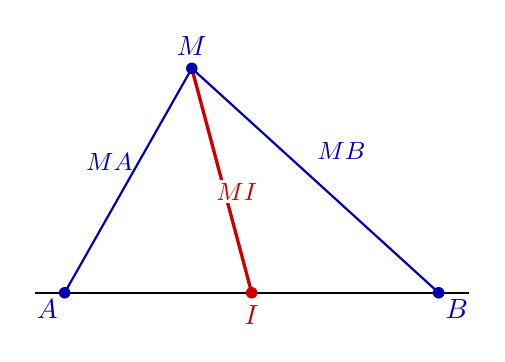
\begin{tikzpicture}[scale=0.95,>=latex]
  \coordinate (A) at (0,0); \coordinate (B) at (5,0); \coordinate (I) at (2.5,0); \coordinate (M) at (1.7,3);
  \draw[thick] (-0.4,0) -- (5.4,0);
  \draw[thick,blue!70!black] (M) -- (A); \draw[thick,blue!70!black] (M) -- (B);
  \draw[very thick,red!80!black] (M) -- (I);
  \fill[blue!70!black] (A) circle (2.2pt) node[below left=-1pt] {$A$};
  \fill[blue!70!black] (B) circle (2.2pt) node[below right=-1pt] {$B$};
  \fill[red!80!black] (I) circle (2.2pt) node[below=1pt] {$I$};
  \fill[blue!70!black] (M) circle (2.2pt) node[above=1pt] {$M$};
  \node[blue!70!black,font=\small] at (0.6,1.75) {$MA$};
  \node[blue!70!black,font=\small] at (3.7,1.9) {$MB$};
  \node[red!80!black,font=\small,fill=white,inner sep=1pt] at (2.3,1.35) {$MI$};
\end{tikzpicture}
